\documentclass[twocolumn]{article}

\usepackage[utf8]{inputenc}
\usepackage[spanish]{babel}
\usepackage{lipsum} % Paquete para generar texto de prueba
\usepackage{graphicx} % Paquete para incluir imágenes
\usepackage{float} % Paquete para posicionar figuras

\title{Práctica 2: Sincronización de procesos con semáforos}
\author{Pedro y Pablo Seijo}
\date{\today}

\begin{document}

\maketitle

\section{Ejercicio 1}

Para forzar las condiciones de carrera, modificamos el código introduciendo sleeps en el productor y el consumidor. Estos sleeps simulan retrasos en la producción y el consumo de elementos, lo que puede llevar a situaciones de carrera si no se sincronizan adecuadamente. A continuación se describen las condiciones de carrera que se pueden producir:

\subsection{Carrera Crítica Productor}

Para esta carrera introducimos un sleep en esta parte del código:

\begin{figure}[H]
    \centering
    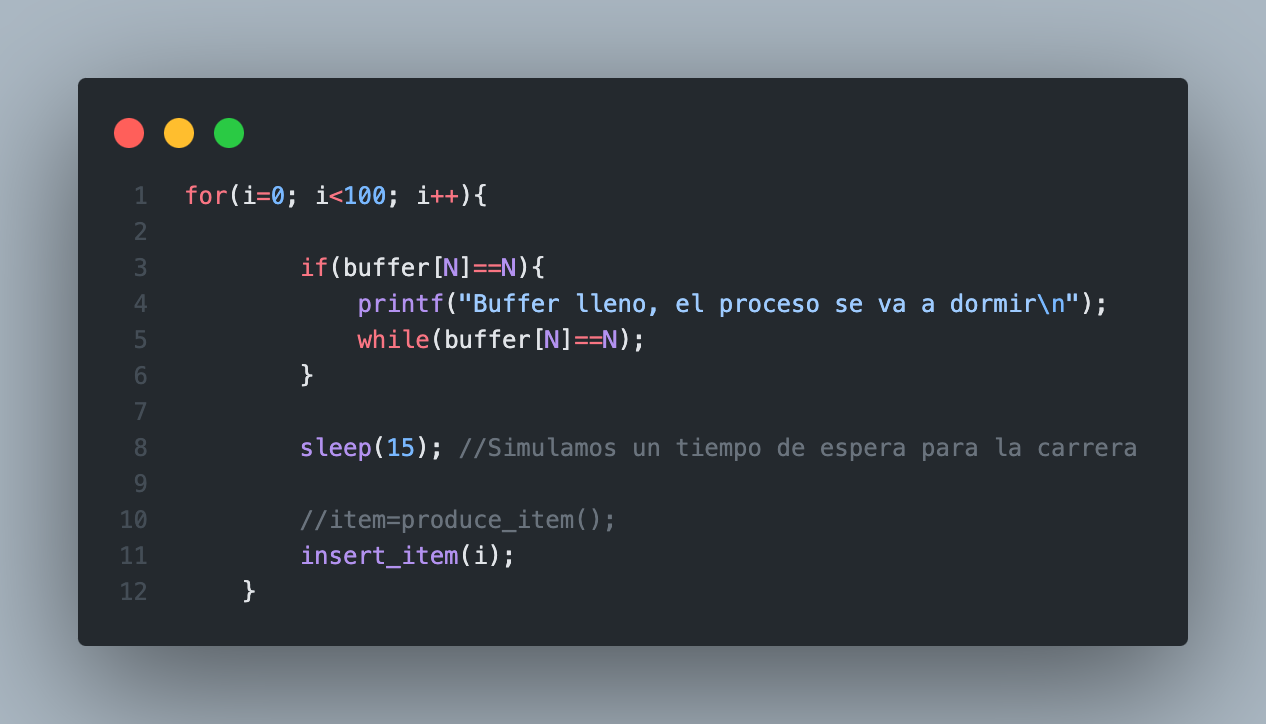
\includegraphics[width=0.5\textwidth]{ejercicio1/productorSleep.png}
    \caption{Código Productor Carrera Crítica} 
    \label{fig:my_label}
\end{figure}

Y la ejecución es la siguiente:

\begin{figure}[H]
    \centering
    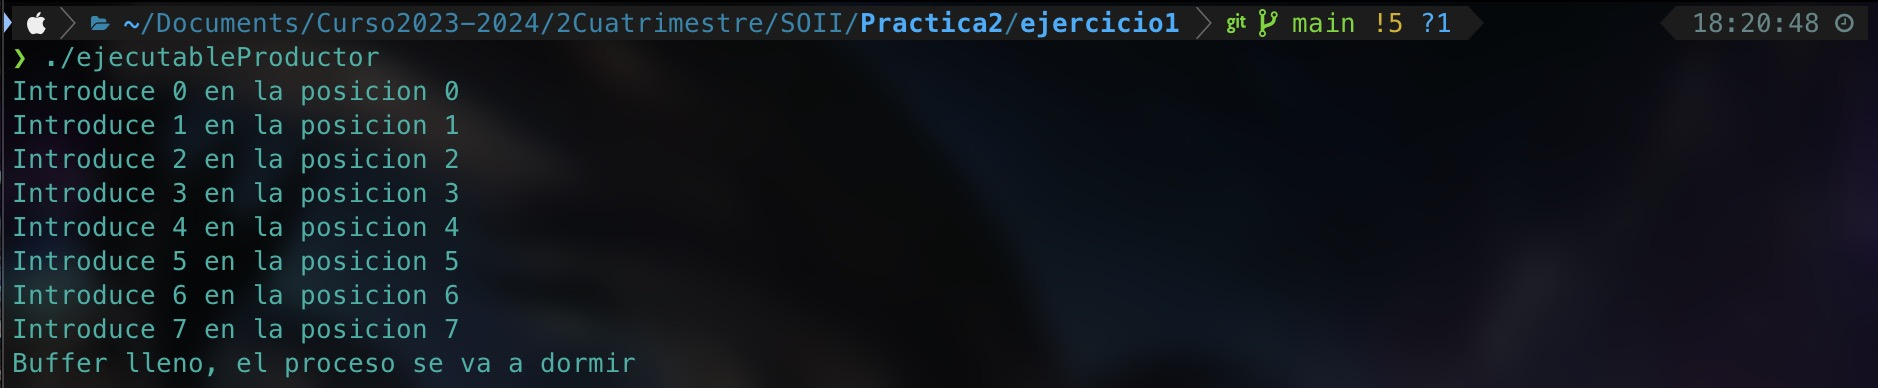
\includegraphics[width=0.5\textwidth]{ejercicio1/productorCarrera.jpg}
    \caption{Carrera Crítica Productor} 
    \label{fig:my_label}
\end{figure}

Aquí, el productor intenta llenar el buffer con nuevos elementos.  Al igual que el consumidor, el productor también emplea una espera activa para verificar el estado del buffer (while(buffer[N]==N);). Si el buffer está lleno, el productor se pone a dormir durante 15 segundos, lo que representa un retraso en la producción de nuevos elementos. Este sueño forzado puede hacer que el productor sea más lento que el consumidor en ciertos momentos, variando la dinámica de producción y consumo y posiblemente llevando a condiciones de carrera si el consumidor se acelera inesperadamente.

\subsection{Carrera Crítica Consumidor}

Para esta carrea introducimos un sleep en esta parte del código:

\begin{figure}[H]
    \centering
    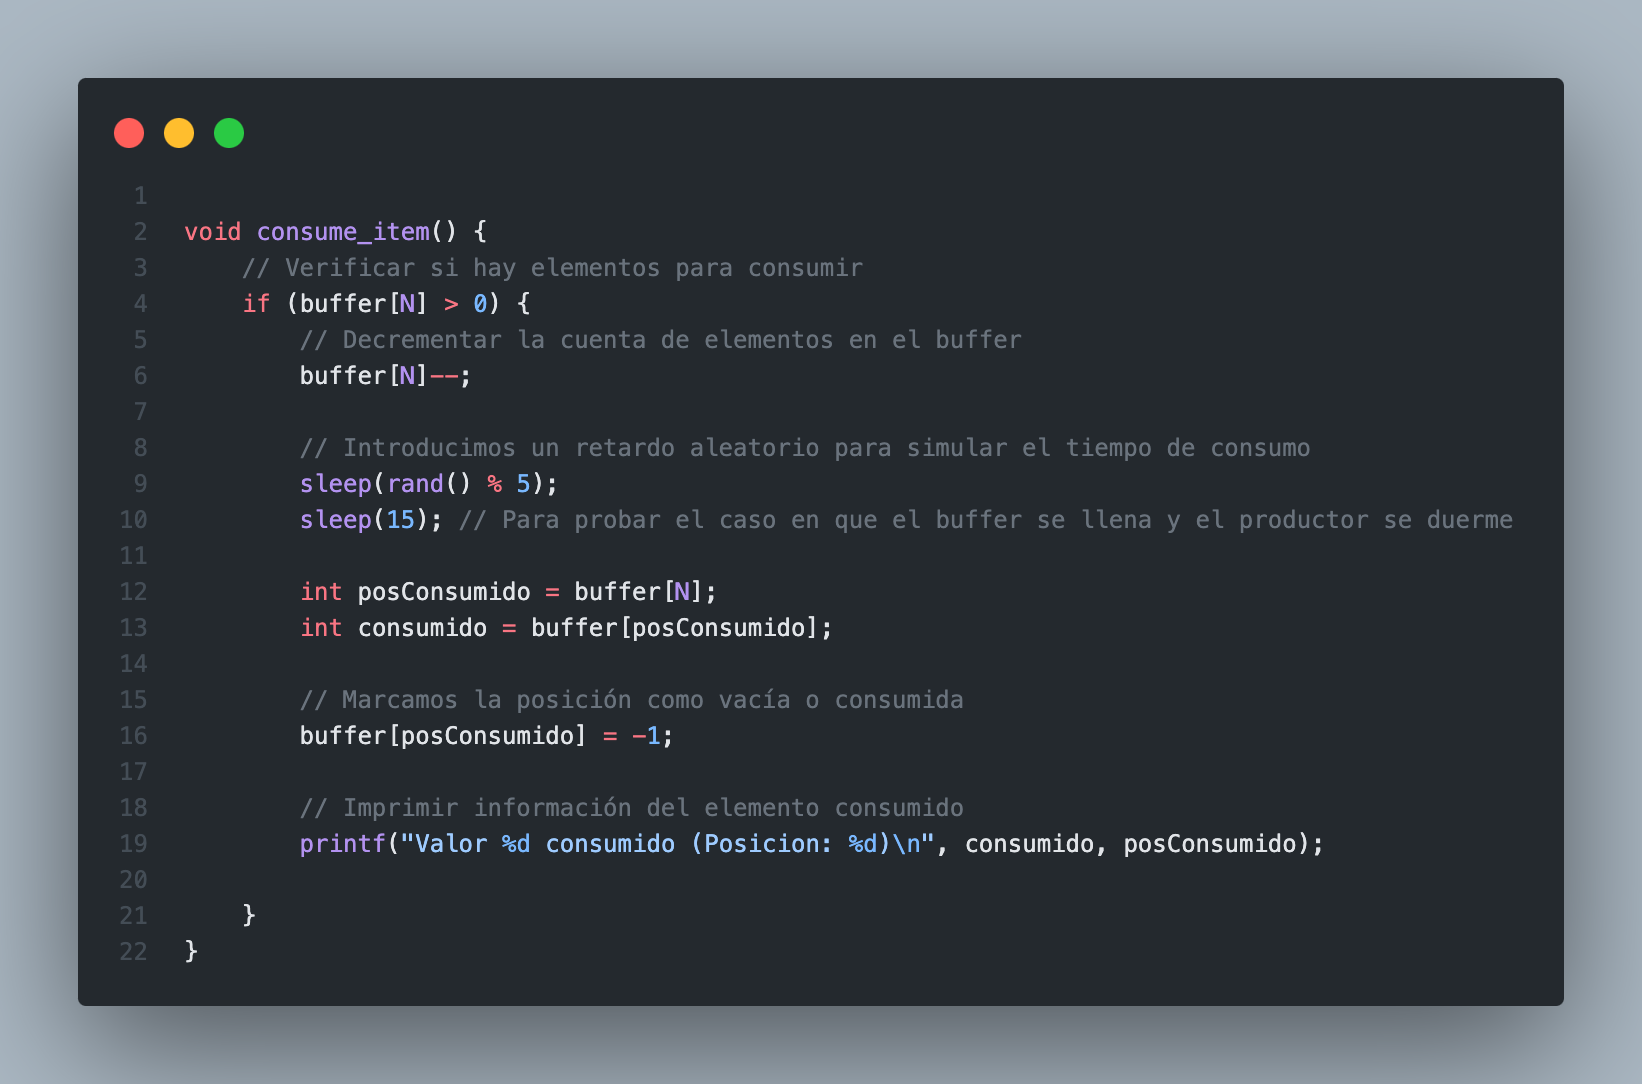
\includegraphics[width=0.5\textwidth]{ejercicio1/consumidorSleep.png}
    \caption{Códugo Carrera Crítica Consumidor} 
    \label{fig:my_label}
\end{figure}

Y la ejecución es la siguiente:

\begin{figure}[H]
    \centering
    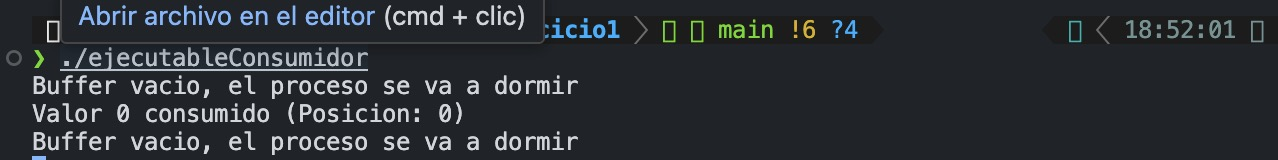
\includegraphics[width=0.5\textwidth]{ejercicio1/consumidorCarrera.jpg}
    \caption{Carrera Crítica Consumidor} 
    \label{fig:my_label}
\end{figure}

De la misma manera en la situación contraria pasa lo siguiente:

\begin{itemize}
    \item El consumidor entra en un estado de espera al detectar que el buffer está vacío. Esta espera se simula mediante una instrucción de suspensión (sleep), durante la cual no hay consumo de elementos.
    
    \item Paralelamente, el productor se activa y comienza a llenar el buffer. Debido a que no hay sincronización, no está consciente de la actividad del consumidor.
    
    \item Si el consumidor sale de su estado de espera y comienza a consumir un elemento al mismo tiempo que el productor está insertando uno, se accede simultáneamente al buffer. Sin mecanismos de sincronización, ambos procesos pueden leer y escribir en la misma posición del buffer o modificar la cuenta de elementos de forma concurrente.
    
    \item Esta simultaneidad puede resultar en que el productor sobrescriba un valor que aún no ha sido consumido o que el consumidor consuma un elemento que el productor cree que ha sido insertado con éxito. Además, la cuenta del buffer (buffer[N]) podría ser incrementada o decrementada incorrectamente, causando desbordamientos o subconsumos.
\end{itemize}

Teniendo en cuenta que una carrera crítica se refiere a un sistema donde su comportamiento final depende de la secuencia o del tiempo de los procesos, y no está controlado por el SO o el programa, sin los controles adecuados, la carrera crítica puede llevar a condiciones de carrera, donde los procesos compiten por recursos compartidos y pueden producir resultados inesperados o indeseados.

\section{Ejercicio 2}

La salida del programa es la siguiente:

\begin{figure}[H]
    \centering
    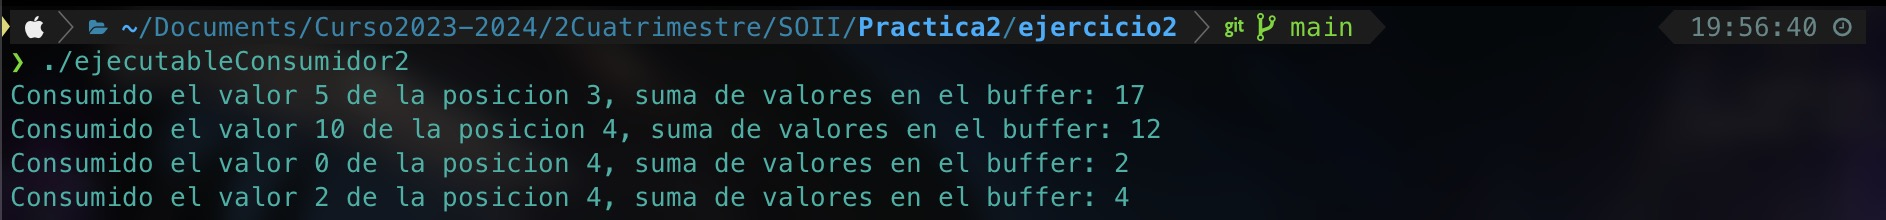
\includegraphics[width=0.5\textwidth]{ejercicio2/consumidor.jpg}
    \caption{Salida del programa de consumidor} 
    \label{fig:my_label}
\end{figure}

\begin{figure}[H]
    \centering
    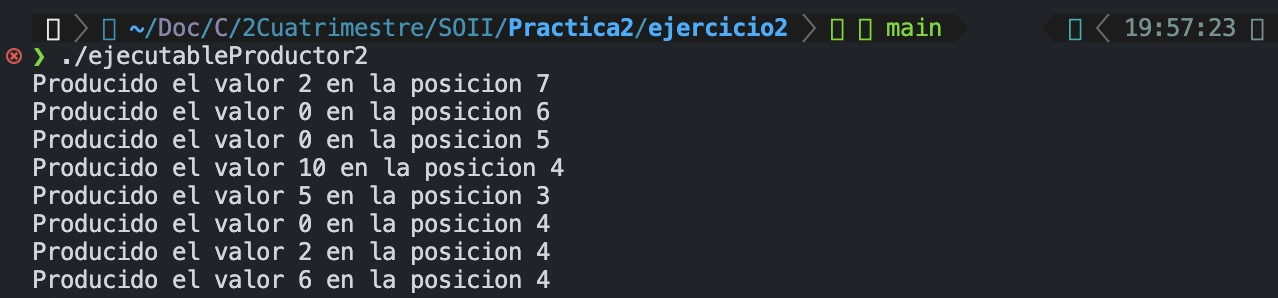
\includegraphics[width=0.5\textwidth]{ejercicio2/productor.jpg}
    \caption{Salida del programa de productor} 
    \label{fig:my_label}
\end{figure}


En este ejercicio se ha implementado una solución al problema del productor-consumidor utilizando memoria compartida y semáforos para gestionar el acceso concurrente a un buffer. Este buffer es de tipo entero (\texttt{int}) y funciona como una pila LIFO (Last In, First Out), donde el último elemento insertado es el primero en ser retirado. La implementación se ha realizado siguiendo estos criterios:

\begin{itemize}
    \item El buffer tiene un tamaño de $N=8$ elementos.
    \item La función \texttt{produce\_item()} genera un entero aleatorio entre 0 y 10 para simular la producción de un elemento.
    \item La función \texttt{insert\_item(int item)} inserta el elemento producido en el buffer siguiendo la política LIFO.
    \item La función \texttt{consume\_item()} retira un elemento del buffer, suma este elemento con todos los valores que haya en el buffer en ese momento, y muestra por pantalla el valor consumido y el resultado de la suma.
\end{itemize}

Se han utilizado semáforos para resolver las carreras críticas, asegurando que sólo un proceso acceda al buffer en un momento dado y gestionando el llenado y vaciado del buffer de manera sincronizada. Los semáforos utilizados son:

\begin{itemize}
    \item Un semáforo llamado \texttt{VACIAS}, inicializado en $N$, que indica el número de posiciones vacías en el buffer.
    \item Un semáforo llamado \texttt{LLENAS}, inicializado en 0, que indica el número de posiciones llenas en el buffer.
    \item Un semáforo de exclusión mutua, \texttt{MUTEX}, inicializado en 1, que asegura el acceso exclusivo al buffer durante las operaciones de inserción y retirada.
\end{itemize}

Para evitar la interrupción del programa en cada ejecución y permitir la observación de la dinámica productor-consumidor, se ha establecido un número finito de iteraciones (100) y se han incluido llamadas a la función \texttt{sleep()} con valores aleatorios entre 0 y 3 segundos, fuera de las regiones críticas, para simular variaciones en las velocidades de producción y consumo.

Finalmente, para asegurar la limpieza y evitar que los semáforos permanezcan activos en el kernel después de la ejecución, se utilizan las funciones \texttt{sem\_close()} y \texttt{sem\_unlink()} al final del programa.

Esta solución demuestra la efectividad de los semáforos para gestionar la sincronización en problemas de concurrencia, permitiendo un control detallado sobre el acceso a recursos compartidos y evitando condiciones de carrera, mientras se mantiene una secuencia ordenada y predecible de operaciones de producción y consumo.

\section{Ejercicio 3}

Ahora se cambia la implementación para utilizar hilos en lugar de procesos. La salida del programa es la siguiente:

\begin{figure}[H]
    \centering
    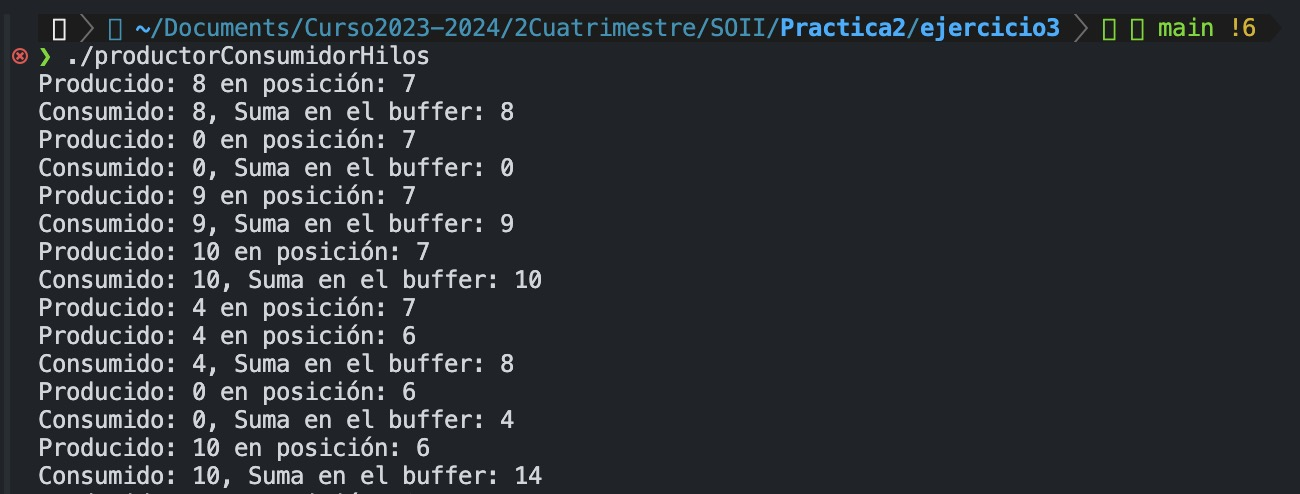
\includegraphics[width=0.5\textwidth]{ejercicio3/salidaHilos.jpg}
    \caption{Salida del programa con hilos} 
    \label{fig:my_label}
\end{figure}

\subsection{Definición y Variables Globales}

El tamaño del buffer se define como $N = 8$, utilizando un arreglo de enteros para simular el buffer. Los semáforos \texttt{vacias}, \texttt{llenas}, y \texttt{mutex} se utilizan para controlar el número de posiciones vacías, el número de posiciones llenas, y asegurar el acceso exclusivo al buffer, respectivamente.

\subsection{Funciones Clave}

\begin{itemize}
    \item \textbf{\texttt{produce\_item()}}: Genera un elemento aleatorio entre 0 y 10.
    \item \textbf{\texttt{insert\_item(int item)}}: Inserta un elemento en el buffer según la política LIFO, decrementando previamente el índice del buffer.
    \item \textbf{\texttt{remove\_item()}}: Elimina un elemento del buffer e imprime el elemento consumido junto con la suma de los valores actuales en el buffer.
\end{itemize}

\subsection{Hilos y Sincronización}

La implementación utiliza dos tipos de hilos: productores y consumidores. Cada productor genera elementos aleatorios y los inserta en el buffer, mientras que cada consumidor retira elementos del buffer. La sincronización se logra mediante el uso de semáforos, donde:

\begin{itemize}
    \item Los semáforos \texttt{vacias} y \texttt{llenas} gestionan el número de posiciones vacías y llenas en el buffer, respectivamente.
    \item El semáforo \texttt{mutex} asegura el acceso exclusivo al buffer para insertar o remover elementos.
\end{itemize}

Los hilos productores esperan que haya posiciones vacías para producir, mientras que los consumidores esperan que el buffer contenga elementos para consumir. Esto asegura que no se produzcan condiciones de carrera y que el acceso al buffer sea seguro y ordenado.


\section{Conclusiones}
\lipsum[7-8] % Texto de prueba

\end{document}